\documentclass[a0,landscape]{a0poster}
%\documentclass[a0,draft]{a0poster}
% With the word preview in the square bracket, your poster will be a4
% size, handy for previewing or submit to x4u queue for A0. 
% with preview removed, you get a file the right size for the HP
% large-format printer. This is a bit bigger than A0, the width is 
% exactly one imperial yard.

% This is so we can have multiple columns of text side-by-side
\usepackage[utf8]{inputenc}
\usepackage{graphicx}
\usepackage{multicol}
\usepackage{helvet}
\usepackage{sectsty}
%\allsectionsfont{\usefont{OT1}{phv}{bc}{n}\selectfont}
\allsectionsfont{\sffamily} \subsubsectionfont{\sffamily\large}
\columnsep=100pt 

% This is the thickness of the black line between the columns of text
\columnseprule=3pt

% this package gives you coloured text and various other simple
% graphics hacks. 
% Details in /usr/local/teTeX/texmf/doc/generic/pstricks/*
\usepackage{pstricks}

%\psset{unit=1cm}

\usepackage{times}
\usepackage{url}

% Define names for some colours 
\newcmykcolor{Inblue}{1.00 0.37 0.00 0.00}
\newcmykcolor{Inred}{0.00 1.00 0.63 0.00}
\newrgbcolor{Inmaroon}{0.4 0.0 0.4}
\newrgbcolor{darkblue}{0.0 0.0 0.5}

% Colour used for figure captions. Change to suit your own preference
\newrgbcolor{captcolor}{0.0 .5 0.0}

\begin{document}

% This is black magic to put a title at the top of the page.
% Thanks to Mark ``the magician'' Filipiak, although I have re-done a
% lot of the code here -- hopefully it is more robust.

% Make a box 0.55* width of poster for title and names
% If your title is long, replace 0.55 with something bigger and 
% make the box for the address smaller by the same amount.
\begin{minipage}[b]{0.65\linewidth} 
\veryHuge \bf 
\textsf{Rapid rule-based machine translation between Dutch and Afrikaans}
\\[1cm]
\huge \bf Pim Otte, Francis M. Tyers,\\
\huge \rm Mendelcollege, Universitat d'Alacant
\end{minipage}
% Make box 0.35 X width of poster for address  
\begin{minipage}[b]{0.35\linewidth} 
\Large Departament de Llenguatges i Sistemes Inform\`{a}tics\\
Universitat d'Alacant\\
E-03071 Alacant\\
Spain\\
\tt{email: ftyers@prompsit.com}
\end{minipage}
%% Make box 0.05*width of poster for EU Shield graphic
%\begin{minipage}[b]{0.05\linewidth}
%\includegraphics[width=10cm]{logo_ofis_liv.pdf}
%%\includegraphics{uitlogo}
%\end{minipage}
\vspace{0.3cm}
\hrule
\vspace{0.3cm}
%\begin{minipage}[b]{\linewidth} 
%\hrule
%{\small \url{http://www.ofis-bzh.org/bzh/ressources_linguistiques/index-troerofis.php}}
%\end{minipage}
%

% This is how many columns your poster will be broken into.
\begin{multicols}{4}

% This is the width your figures will be scaled to. Change this if you 
% change the number of columns.
\newlength{\figwidth}
\setlength{\figwidth}{20cm}

% Set to half of figwidth. Used for putting two figs side by side
\newlength{\fighalfwidth}
\setlength{\fighalfwidth}{10cm}

% Can't use the figure environment within multicolumns. Set up our own 
% counter for figures.
\newcounter{figscount}

\section{Introduction}

\noindent
{\bf Dutch} is a West-Germanic language spoken by nearly 23 million people, mostly from the 
Netherlands and Flanders. {\bf Afrikaans} is spoken by at least 5 million people, mainly in 
South-Africa,but also in Namibia. Afrikaans is a variety of Dutch that originates from that 
spoken by the the Dutch colonists of the Cape Colony. In 1925 Afrikaans replaced Dutch as
an official language in South-Africa, to be the joint official language together with English.
In this paper we will describe the development of {\small {\tt apertium-af-nl}}, a bi-directional Afrikaans 
and Dutch machine-translation system

\vspace{0.5cm}

\section{Method}

\noindent
The system is based on {\bf Apertium} (\url{http://www.apertium.org/}), a free/open-source rule-based
machine translation platform. To create the language pair we used an existing resource and created 
several new ones. \\

\begin{center}
\begin{minipage}[b]{26cm}
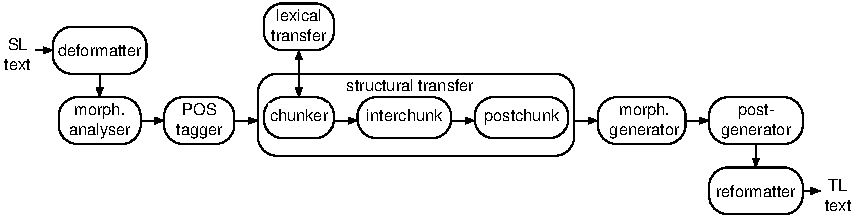
\includegraphics[width=260mm]{apertium2.pdf}
\end{minipage}\\
\textbf{Figure 1:} Modules of the Apertium translation system
\vspace{0.3cm}
\end{center}


\vspace{0.5cm}

\subsection{Existing resources}

\noindent
We reused the morphological transducer for Afrikaans, created during a currently dormant English-Afrikaans
Machine Translation project.\\

\subsection{Resources created}

\subsubsection{Dutch morphological transducer}
A new Dutch morphological transducer was created, because existing ones were unsuitable for several reasons:

\begin{itemize}
 \item Non-free license
 \item Not bidirectional
 \item Tagset different from Afrikaans transducer
\end{itemize}

\vspace{0.5cm}

\noindent
The open categories (nouns, verbs, adjectives, adverbs) for the Dutch 
morphological analyser were extracted semi-automatically from 
Wiktionary, (\url{http://www.wiktionary.org}), which has entries like in {\bf Figure 2}
Closed categories were added by hand based on a grammar of Dutch.
\vspace{0.5cm}

\begin{center}
\begin{minipage}[b]{26cm}
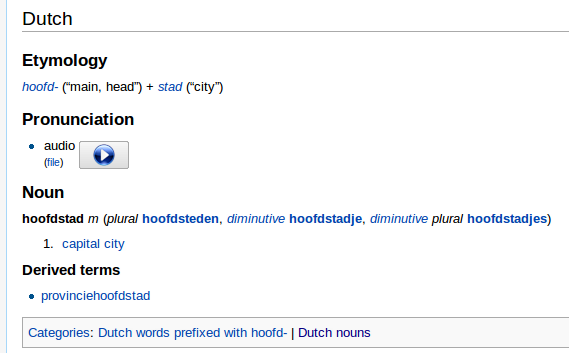
\includegraphics[width=260mm]{hoofdstad.png}
\end{minipage}\\
\textbf{Figure 2:} Example of Wiktionary entry: Hoofdstad
\label{wikt1}
\vspace{0.3cm}
\end{center}


\vspace{0.5cm}

\noindent
The analyser has a coverage of between 87--90\% over two free corpora of Breton (Wikipedia and \emph{Bremaik}).

\subsubsection{Bilingual dictionary}

\noindent
The bilingual dictionary was developed by adding exact matches, extracting proper names
from Wikipedia, adding cognates, words which often have a small spelling difference and adding
some entries by hand, such as closed categories and frequently missing words.

\subsection{Transfer rules}
Several transfer rules were added.

\subsubsection{Afrikaans to Dutch}
An example of an Afrikaans to Dutch transfer rule, which handles the auxiliary verb, can be seen in
{\bf Figure 3}

\begin{center}
\begin{minipage}[b]{25cm}
\begin{small}
\begin{verbatim}
    <rule comment="REGLA: nie">
      <pattern>
        <pattern-item n="nie"/>
      </pattern>
      <action>
        <choose>
          <when>
            <test>
              <equal>
                <var n="seen_neg"/>
                <lit v="true"/>
              </equal>
            </test>
          </when>
          <otherwise>
            <out>
              <chunk name="nie">
                <tags>
                  <tag><lit-tag v="ADV"/></tag>
                </tags>
                <lu>
                  <clip pos="1" side="tl" part="lemh"/>
                  <clip pos="1" side="tl" part="a_adv"/>
                  <clip pos="1" side="tl" part="lemq"/>
                </lu>
              </chunk>
            </out>
          </otherwise>
        </choose>
        <let>
         <var n="seen_neg"/>
         <lit v="true"/>
        </let>
      </action>
    </rule>
\end{verbatim}
\end{small}
\end{minipage}\\
~\\
\textbf{Figure 3:} Transfer rule for the pattern "have + past participle"
\vspace{0.5cm}
\end{center}

\subsubsection{Compound words}
In both Afrikaans and Dutch words can combine very productively into compounds.
{\small {\tt apertium-af-nl}} can handle compounds that consist of one or more nouns, 
such as the one in {\bf Figure 4}. \\

\begin{center}
\begin{minipage}[b]{26cm}
\begin{small}
\begin{verbatim}
lugmag

^lug<n><sg><cmp>+mag<n><sg>$

^lucht<n><mf><sg><cmp>$^macht<n><mf><sg>$

luchtmacht
\end{verbatim}
\end{small}
\end{minipage}\\
\end{center}
~\\
\textbf{Figure 4:} Example of compound analysis: lugmag (air force)



\subsection{Seperable verbs}

\noindent
The system can handle seperable verbs, which exist both in Afrikaans and Dutch, as
long as there are no other phrases between the seperated parts.\\

\section{Evaluation}
\noindent
We evaluated the system in several ways: Naïve coverage, compound analysis, qualitative, quantitative and comparative

\subsection{Coverage}

\noindent
Naïve coverage was calculated over Wikipedia corpora.\\


\begin{minipage}[b]{25cm}
\begin{center}
  \begin{tabular}{|l|r|r|}
   \hline
   {\bf Corpus}           & {\bf Tokens}    & {\bf Coverage}\\
   \hline
   {\tt af} Wikipedia     & 2,926,943       & 82.1\% $\pm$ 0.8 \\
   \hline
   {\tt nl} Wikipedia     & 18,569,183      & 80.5\% $\pm$ 0.7 \\
   \hline
  \end{tabular}
    
 \end{center}
 \textbf{Table 1:} Na\"ive vocabulary coverage for the two morphological analysers.
\end{minipage}\\

\subsection{Compound words}
\noindent
To test the accuracy of the compound word analysis, we marked words as correctly segmented and/or 
correctly translated, this test was performed in the Afrikaans$\rightarrow$Dutch direction.

\begin{minipage}[b]{25cm}
  \begin{center}
  \begin{tabular}{|l|r|r|}
   \hline
   {\bf Corpus}    & {\bf Corr. Seg.}    & {\bf Corr. Trans.}\\
   \hline
   top-1,000       & 914                 &  776 \\ 
   \hline
   random-1,000    & 957                 &  801 \\ 
   \hline
  \end{tabular}
  \end{center}
  \textbf{Table 2:} Compound word accuracy in analysis and translation.
\end{minipage}\\




\end{multicols}
\end{document}

